\documentclass[tikz,border=10pt]{standalone}
\begin{document}
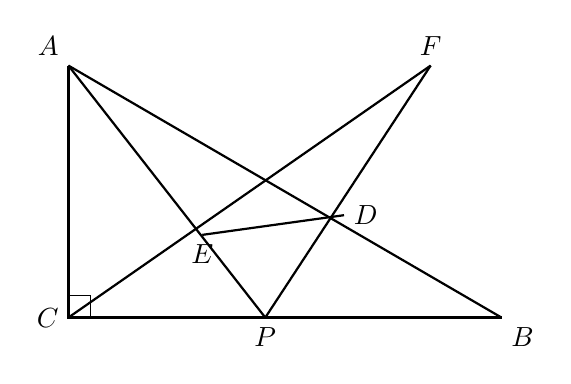
\begin{tikzpicture}
\coordinate (A) at (0,3.2);
\coordinate (C) at (0,0);
\coordinate (B) at (5.5,0);
\coordinate (P) at (2.5,0);
\coordinate (E) at (1.7,1.05);
\coordinate (D) at (3.5,1.3);
\coordinate (F) at (4.6,3.2);

\draw[thick] (A) -- (C) -- (B);
\draw[thick] (A) -- (P);
\draw[thick] (A) -- (B);
\draw[thick] (C) -- (F);
\draw[thick] (P) -- (F);
\draw[thick] (E) -- (D);

\draw (0,0.28) -- (0.28,0.28) -- (0.28,0);

\node[above left] at (A) {$A$};
\node[left] at (C) {$C$};
\node[below right] at (B) {$B$};
\node[below] at (P) {$P$};
\node[below] at (E) {$E$};
\node[right] at (D) {$D$};
\node[above] at (F) {$F$};
\end{tikzpicture}
\end{document}
